\documentclass[aspectratio=169,11pt]{beamer}
\usepackage[T1]{fontenc}
\usepackage{lmodern,amsmath,amssymb,tikz}
\usetikzlibrary{arrows.meta,positioning,calc,decorations.pathreplacing,shapes.geometric}
\definecolor{bluefam}{RGB}{30,105,175}
\definecolor{orangefam}{RGB}{195,87,20}
\definecolor{target}{RGB}{35,133,87}
\definecolor{corner}{RGB}{132,69,160}
\definecolor{gold}{RGB}{216,164,37}
\definecolor{ink}{RGB}{33,46,65}
\definecolor{soft}{RGB}{243,246,250}
\usetheme{default}
\setbeamertemplate{navigation symbols}{}
\setbeamertemplate{footline}{\hfill\color{ink!65}\small\insertframenumber/\inserttotalframenumber\hspace{4mm}\vspace{2mm}}
\setbeamercolor{frametitle}{fg=ink}
\setbeamerfont{frametitle}{series=\bfseries,size=\Large}
\setbeamercolor{structure}{fg=bluefam}
\setbeamercolor{block title}{fg=ink,bg=bluefam!12}
\setbeamercolor{block body}{fg=ink,bg=soft}
\setbeamercolor{block title alerted}{fg=ink,bg=orangefam!17}
\setbeamercolor{block body alerted}{fg=ink,bg=orangefam!5}
\ifdefined\SpeakerNotes
\setbeameroption{show only notes}
\else
\setbeameroption{hide notes}
\fi
\newcommand{\abs}[1]{\lvert#1\rvert}
\newcommand{\takeaway}[1]{\par\medskip{\color{bluefam!85!black}\bfseries #1}\par}
\tikzset{
 vertex/.style={circle,draw=ink,fill=white,minimum size=6mm,inner sep=1pt},
 arc/.style={-{Stealth[length=2mm]},thick},
 stage/.style={draw=ink!65,rounded corners,align=center,text width=32mm,minimum height=18mm,inner sep=5pt,font=\small},
 leftpt/.style={circle,draw=bluefam!80!black,fill=bluefam,minimum size=4mm,inner sep=0pt},
 rightpt/.style={rectangle,draw=orangefam!80!black,fill=orangefam,minimum size=3.8mm,inner sep=0pt},
 targetpt/.style={diamond,draw=target!80!black,fill=target,minimum size=4.8mm,inner sep=0pt},
 starpt/.style={star,star points=5,draw=corner!80!black,fill=corner,minimum size=5.5mm,inner sep=0pt}}
% New Codex vector diagrams, November 15. Shared conventions are in talk.tex.
\newcommand{\NeighborhoodPicture}{%
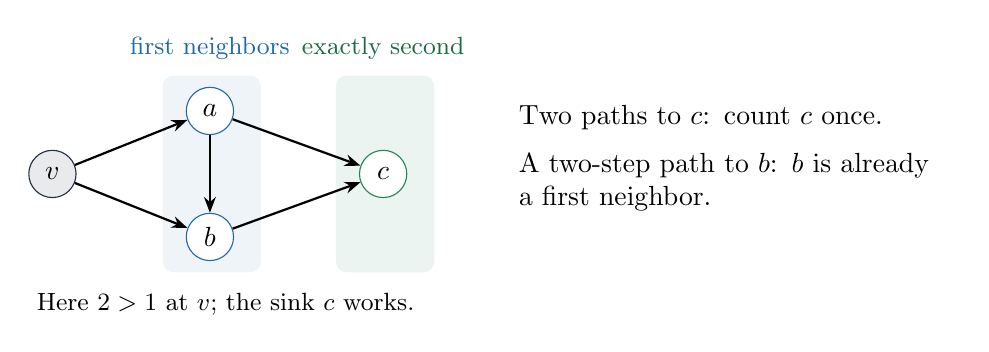
\begin{tikzpicture}
\fill[bluefam!7,rounded corners] (1.4,-1.25) rectangle (2.65,1.25);
\fill[target!9,rounded corners] (3.6,-1.25) rectangle (4.85,1.25);
\node[vertex,fill=ink!10] (v) at (0,0) {$v$};
\node[vertex,draw=bluefam] (a) at (2,0.8) {$a$};
\node[vertex,draw=bluefam] (b) at (2,-0.8) {$b$};
\node[vertex,draw=target] (c) at (4.2,0) {$c$};
\draw[arc] (v)--(a);\draw[arc] (v)--(b);\draw[arc] (a)--(b);
\draw[arc] (a)--(c);\draw[arc] (b)--(c);
\node[font=\small,bluefam] at (2,1.6) {first neighbors};
\node[font=\small,target!80!black] at (4.2,1.6) {exactly second};
\node[align=left,text width=55mm,anchor=west] at (5.8,0.2)
{Two paths to $c$: count $c$ once.\\[5pt]A two-step path to $b$: $b$ is already a first neighbor.};
\node[font=\small] at (2.2,-1.65) {Here $2>1$ at $v$; the sink $c$ works.};
\end{tikzpicture}}

\newcommand{\ProofMap}{%
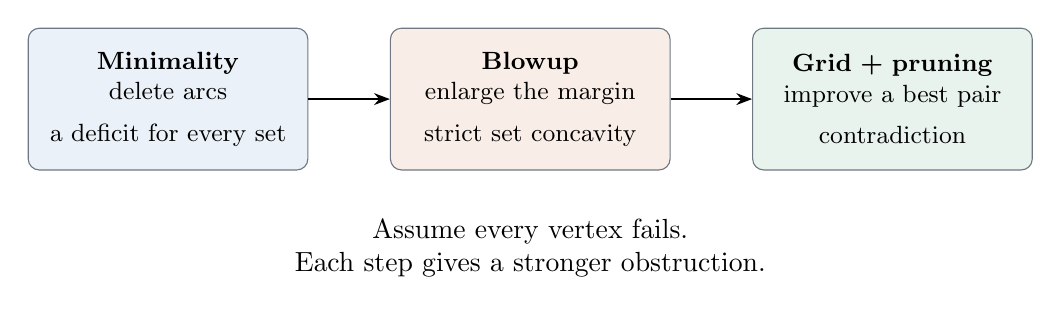
\begin{tikzpicture}
\node[stage,fill=bluefam!9] (a) at (0,0) {\textbf{Minimality}\\delete arcs\\[4pt]a deficit for every set};
\node[stage,fill=orangefam!10] (b) at (4.6,0) {\textbf{Blowup}\\enlarge the margin\\[4pt]strict set concavity};
\node[stage,fill=target!10] (c) at (9.2,0) {\textbf{Grid + pruning}\\improve a best pair\\[4pt]contradiction};
\draw[arc] (a)--(b);\draw[arc] (b)--(c);
\node[anchor=north,align=center,text width=11cm] at (4.6,-1.4)
{Assume every vertex fails.\\Each step gives a stronger obstruction.};
\end{tikzpicture}}

\newcommand{\DeletionPicture}{%
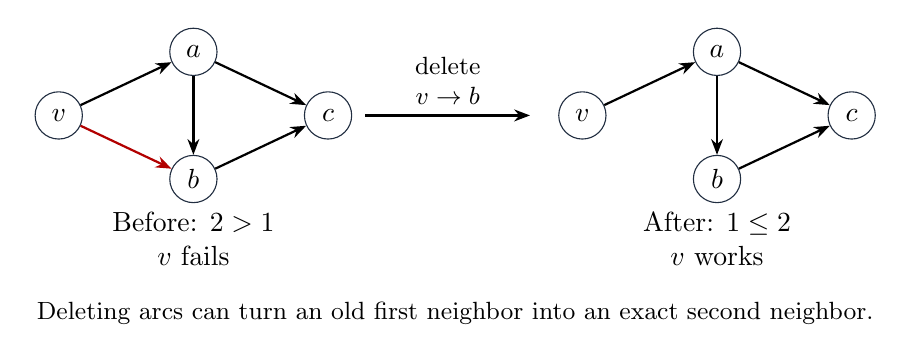
\begin{tikzpicture}[scale=0.95]
\foreach \shift/\tag in {0/old,7/new}{
\begin{scope}[xshift=\shift cm]
\node[vertex] (v\tag) at (0,0) {$v$};
\node[vertex] (a\tag) at (1.8,.85) {$a$};
\node[vertex] (b\tag) at (1.8,-.85) {$b$};
\node[vertex] (c\tag) at (3.6,0) {$c$};
\draw[arc] (v\tag)--(a\tag);\draw[arc] (a\tag)--(b\tag);
\draw[arc] (a\tag)--(c\tag);\draw[arc] (b\tag)--(c\tag);
\end{scope}}
\draw[arc,red!70!black] (vold)--(bold);
\draw[arc,line width=1.2pt] (4.1,0)--node[above,font=\small,align=center] {delete\\$v\to b$} (6.3,0);
\node[align=center] at (1.8,-1.65) {Before: $2>1$\\$v$ fails};
\node[align=center] at (8.8,-1.65) {After: $1\le2$\\$v$ works};
\node[font=\small,align=center] at (5.3,-2.65)
{Deleting arcs can turn an old first neighbor into an exact second neighbor.};
\end{tikzpicture}}

\newcommand{\BatchPicture}{%
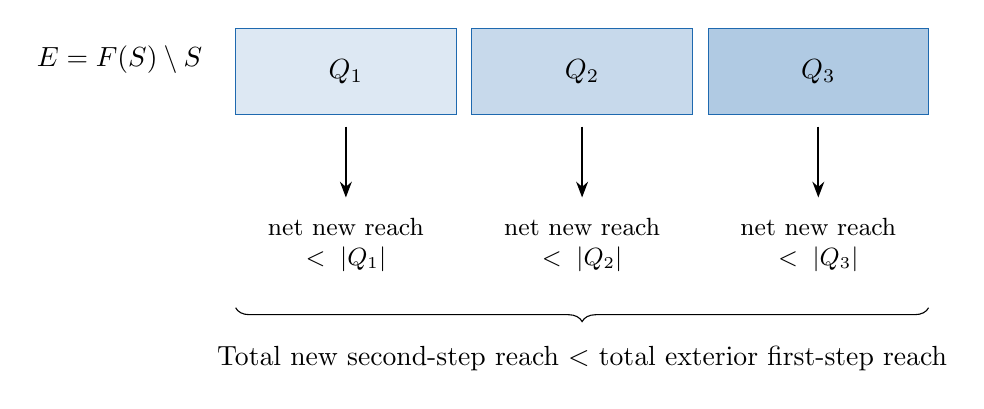
\begin{tikzpicture}
\node[anchor=east] at (-.3,.7) {$E=F(S)\setminus S$};
\foreach \x/\q/\shade in {0/1/15,3/2/25,6/3/35}{
\draw[fill=bluefam!\shade,draw=bluefam] (\x,0) rectangle ++(2.8,1.1);
\node at (\x+1.4,.55) {$Q_{\q}$};
\draw[arc] (\x+1.4,-.15)--(\x+1.4,-1.05);
\node[align=center,font=\small,text width=24mm] at (\x+1.4,-1.65)
{net new reach\\$<|Q_{\q}|$};}
\draw[decorate,decoration={brace,amplitude=5pt,mirror}] (0,-2.45)--(8.8,-2.45);
\node at (4.4,-3.1) {Total new second-step reach $<$ total exterior first-step reach};
\end{tikzpicture}}

\newcommand{\BlowupPicture}{%
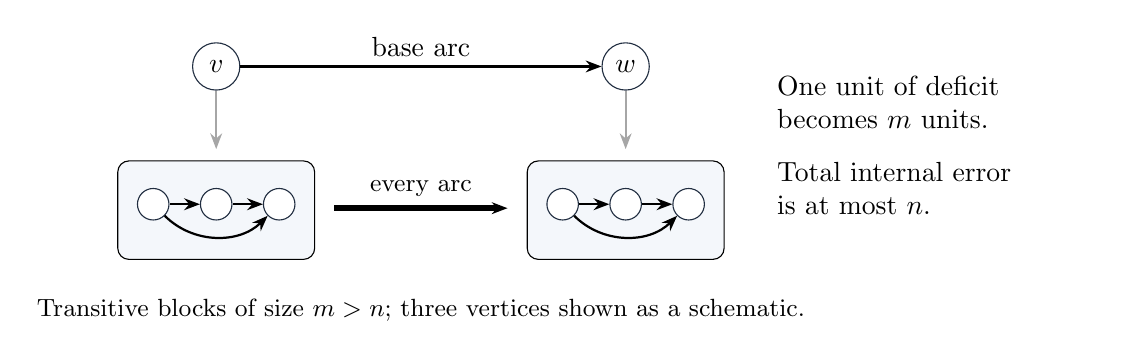
\begin{tikzpicture}
\node[vertex] (v) at (0,1.3) {$v$};\node[vertex] (w) at (5.2,1.3) {$w$};
\draw[arc] (v)--node[above] {base arc} (w);
\draw[arc,black!35] (v)--(0,.25);\draw[arc,black!35] (w)--(5.2,.25);
\foreach \shift/\tag in {0/v,5.2/w}{
\begin{scope}[xshift=\shift cm]
\draw[rounded corners,fill=bluefam!5] (-1.25,-1.15) rectangle (1.25,.1);
\foreach \x/\n in {-.8/1,0/2,.8/3} {\node[vertex,minimum size=4mm] (\tag\n) at (\x,-.45) {};}
\draw[arc] (\tag1)--(\tag2);\draw[arc] (\tag2)--(\tag3);
\draw[arc] (\tag1) to[bend right=45] (\tag3);
\end{scope}}
\draw[arc,line width=2pt] (1.5,-.5)--node[above,font=\small] {every arc} (3.7,-.5);
\node[align=left,anchor=west,text width=40mm] at (7,.3)
{One unit of deficit\\becomes $m$ units.\\[7pt]Total internal error\\is at most $n$.};
\node[font=\small] at (2.6,-1.8) {Transitive blocks of size $m>n$; three vertices shown as a schematic.};
\end{tikzpicture}}

\newcommand{\ConcavityPicture}{%
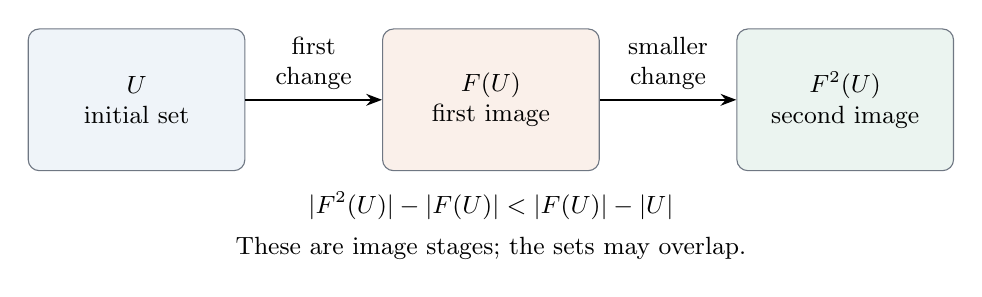
\begin{tikzpicture}
\node[stage,minimum width=25mm,text width=24mm,fill=bluefam!7] (s) at (0,0) {$U$\\initial set};
\node[stage,minimum width=25mm,text width=24mm,fill=orangefam!9] (f) at (4.5,0) {$F(U)$\\first image};
\node[stage,minimum width=25mm,text width=24mm,fill=target!9] (ff) at (9,0) {$F^2(U)$\\second image};
\draw[arc] (s)--node[above,font=\small,align=center] {first\\change} (f);
\draw[arc] (f)--node[above,font=\small,align=center] {smaller\\change} (ff);
\node[align=center,font=\small] at (4.5,-1.6)
{$|F^2(U)|-|F(U)|<|F(U)|-|U|$\\[4pt]These are image stages; the sets may overlap.};
\end{tikzpicture}}

% Exact board for the directed cycle 1 -> 2 -> 3 -> 1.
\newcommand{\CycleBoard}{%
\foreach \i in {1,2,3}{
\node[font=\small] at (.25,-\i) {$\i$};\node[font=\small] at (\i,-.25) {$\i$};
\foreach \j in {1,2,3}{\draw[black!25] (\j-.45,-\i-.45) rectangle ++(.9,.9);}}
\foreach \i/\j in {2/1,3/2,1/3}{\node[leftpt] at (\j,-\i) {};}
\foreach \i/\j in {1/2,2/3,3/1}{\node[rightpt] at (\j,-\i) {};}
\foreach \k in {1,2,3}{\node[circle,fill=ink,minimum size=3mm,inner sep=0pt] (d\k) at (\k,-\k) {};}}

\newcommand{\WhyGridPicture}{%
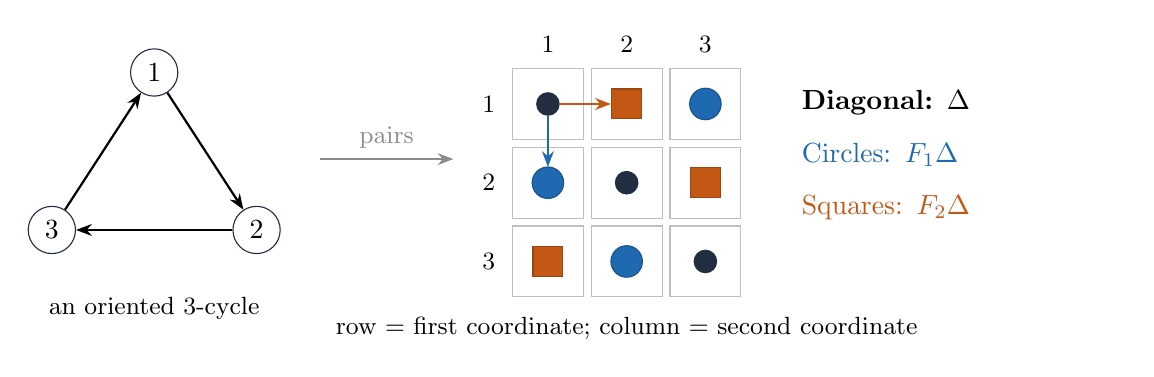
\begin{tikzpicture}
\node[vertex] (v1) at (0,-.6) {$1$};
\node[vertex] (v2) at (1.3,-2.6) {$2$};\node[vertex] (v3) at (-1.3,-2.6) {$3$};
\draw[arc] (v1)--(v2);\draw[arc] (v2)--(v3);\draw[arc] (v3)--(v1);
\node[font=\small] at (0,-3.6) {an oriented $3$-cycle};
\draw[arc,black!45] (2.1,-1.7)--node[above,font=\small] {pairs} (3.8,-1.7);
\begin{scope}[xshift=4cm]\CycleBoard
\draw[arc,bluefam] (d1)--(1,-1.8);
\draw[arc,orangefam] (d1)--(1.8,-1);
\end{scope}
\node[anchor=west,align=left,text width=4cm] at (8.1,-1.65)
{\textbf{Diagonal:} $\Delta$\\[7pt]\textcolor{bluefam}{Circles: $F_1\Delta$}\\[7pt]\textcolor{orangefam}{Squares: $F_2\Delta$}};
\node[font=\small] at (6,-3.85) {row = first coordinate; column = second coordinate};
\end{tikzpicture}}

\newcommand{\ScorePicture}{%
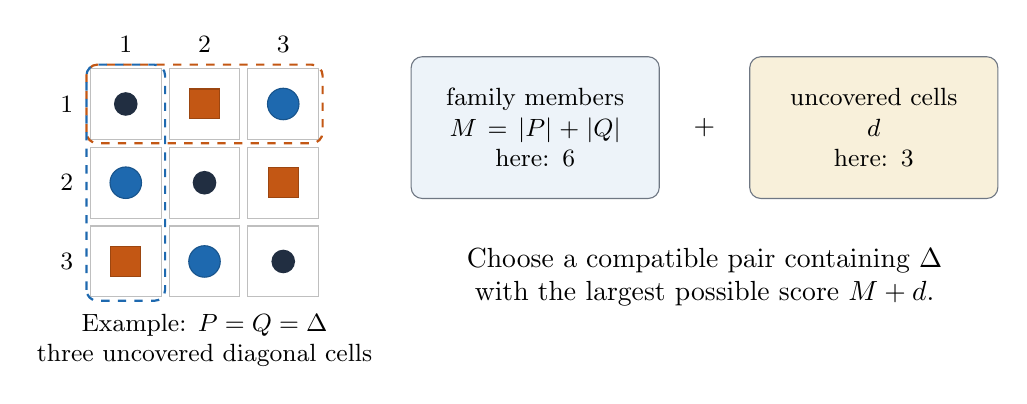
\begin{tikzpicture}
\begin{scope}\CycleBoard\end{scope}
\draw[orangefam,dashed,thick,rounded corners] (.5,-1.5) rectangle (3.5,-.5);
\draw[bluefam,dashed,thick,rounded corners] (.5,-3.5) rectangle (1.5,-.5);
\node[align=center,font=\small] at (2,-4) {Example: $P=Q=\Delta$\\three uncovered diagonal cells};
\node[stage,text width=28mm,fill=bluefam!8] (m) at (6.2,-1.3)
{family members\\$M=|P|+|Q|$\\here: $6$};
\node at (8.35,-1.3) {$+$};
\node[stage,text width=28mm,fill=gold!17] (d) at (10.5,-1.3)
{uncovered cells\\$d$\\here: $3$};
\node[align=center] at (8.35,-3.2) {Choose a compatible pair containing $\Delta$\\with the largest possible score $M+d$.};
\end{tikzpicture}}

\newcommand{\ImprovementPicture}{%
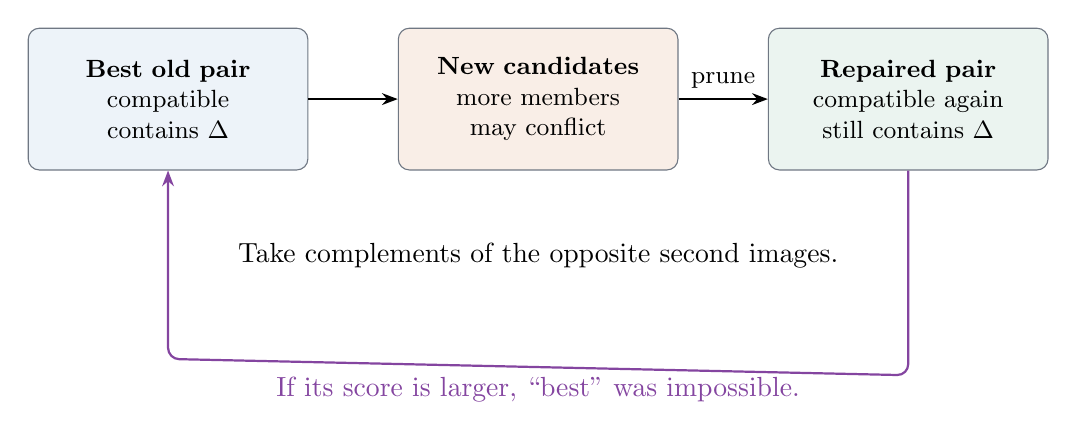
\begin{tikzpicture}
\node[stage,fill=bluefam!8] (a) at (0,0) {\textbf{Best old pair}\\compatible\\contains $\Delta$};
\node[stage,fill=orangefam!10] (b) at (4.7,0) {\textbf{New candidates}\\more members\\may conflict};
\node[stage,fill=target!9] (c) at (9.4,0) {\textbf{Repaired pair}\\compatible again\\still contains $\Delta$};
\draw[arc] (a)--(b);
\draw[arc] (b)--node[above,font=\small] {prune} (c);
\node[below=8mm of b,align=center] (w) {Take complements of the opposite second images.};
\draw[arc,corner,rounded corners] (c.south)--++(0,-2.6)--node[below] {If its score is larger, ``best'' was impossible.} (0,-3.3)--(a.south);
\end{tikzpicture}}

\newcommand{\RectanglePicture}{%
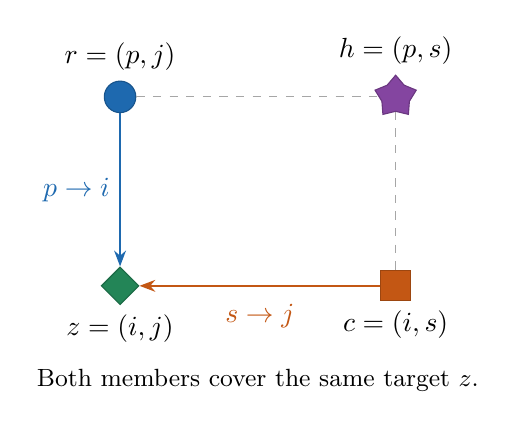
\begin{tikzpicture}
\node[leftpt,label=above:{$r=(p,j)$}] (r) at (0,0) {};
\node[starpt,label=above:{$h=(p,s)$}] (h) at (3.5,0) {};
\node[targetpt,label=below:{$z=(i,j)$}] (z) at (0,-2.4) {};
\node[rightpt,label=below:{$c=(i,s)$}] (c) at (3.5,-2.4) {};
\draw[arc,bluefam] (r)--node[left] {$p\to i$} (z);
\draw[arc,orangefam] (c)--node[below=3pt] {$s\to j$} (z);
\draw[black!35,dashed] (r)--(h)--(c);
\node[font=\small] at (1.75,-3.6) {Both members cover the same target $z$.};
\end{tikzpicture}}

\newcommand{\PruningExamplePicture}{%
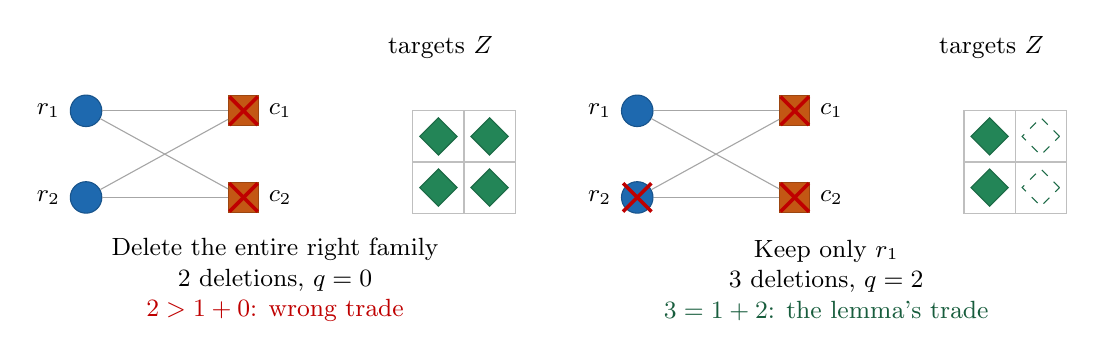
\begin{tikzpicture}[font=\small]
\foreach \shift/\mode in {0/1,7/2}{
\begin{scope}[xshift=\shift cm]
\node[leftpt,label=left:{$r_1$}] (r1\mode) at (0,0) {};
\node[leftpt,label=left:{$r_2$}] (r2\mode) at (0,-1.1) {};
\node[rightpt,label=right:{$c_1$}] (c1\mode) at (2,0) {};
\node[rightpt,label=right:{$c_2$}] (c2\mode) at (2,-1.1) {};
\foreach \a in {1,2}\foreach \b in {1,2}{\draw[black!35] (r\a\mode)--(c\b\mode);}
\foreach \b in {1,2}{
\draw[red!75!black,line width=1.3pt] ($(c\b\mode)+(-.18,-.18)$)--($(c\b\mode)+(.18,.18)$);
\draw[red!75!black,line width=1.3pt] ($(c\b\mode)+(-.18,.18)$)--($(c\b\mode)+(.18,-.18)$);}
\ifnum\mode=2
\draw[red!75!black,line width=1.3pt] ($(r2\mode)+(-.18,-.18)$)--($(r2\mode)+(.18,.18)$);
\draw[red!75!black,line width=1.3pt] ($(r2\mode)+(-.18,.18)$)--($(r2\mode)+(.18,-.18)$);
\fi
\node at (4.5,.8) {targets $Z$};
\foreach \i in {1,2}\foreach \j in {1,2}{
\draw[black!25] (3.5+\j*.65,-\i*.65+.65) rectangle ++(.65,-.65);
\ifnum\mode=1
\node[targetpt] at (3.825+\j*.65,-\i*.65+.325) {};
\else
\ifnum\j=1
\node[targetpt] at (3.825+\j*.65,-\i*.65+.325) {};
\else
\node[targetpt,fill=white,dashed] at (3.825+\j*.65,-\i*.65+.325) {};
\fi\fi}
\end{scope}}
\node[align=center] at (2.4,-2.15) {Delete the entire right family\\$2$ deletions, $q=0$\\\textcolor{red!75!black}{$2>1+0$: wrong trade}};
\node[align=center] at (9.4,-2.15) {Keep only $r_1$\\$3$ deletions, $q=2$\\\textcolor{target!70!black}{$3=1+2$: the lemma's trade}};
\end{tikzpicture}}

\newcommand{\CoverPicture}{%
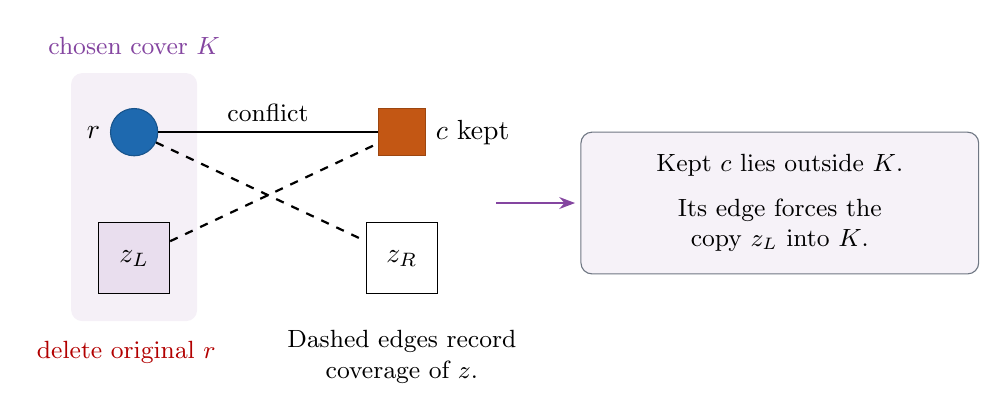
\begin{tikzpicture}
\fill[corner!8,rounded corners] (-.8,1.35) rectangle (.8,-1.8);
\node[font=\small,corner] at (0,1.7) {chosen cover $K$};
\node[leftpt,minimum size=6mm,label=left:{$r$}] (r) at (0,.6) {};
\node[draw,rectangle,fill=corner!18,minimum size=9mm] (zl) at (0,-1) {$z_L$};
\node[rightpt,minimum size=6mm,label=right:{$c$ kept}] (c) at (3.4,.6) {};
\node[draw,rectangle,minimum size=9mm] (zr) at (3.4,-1) {$z_R$};
\draw[thick] (r)--node[above,font=\small] {conflict} (c);
\draw[thick,dashed] (r)--(zr);\draw[thick,dashed] (zl)--(c);
\node[red!70!black,font=\small] at (-.1,-2.2) {delete original $r$};
\node[font=\small,align=center] at (3.4,-2.25) {Dashed edges record\\coverage of $z$.};
\draw[arc,corner] (4.6,-.3)--(5.6,-.3);
\node[stage,text width=47mm,fill=corner!7] at (8.2,-.3)
{Kept $c$ lies outside $K$.\\[5pt]Its edge forces the copy $z_L$ into $K$.};
\end{tikzpicture}}

\newcommand{\AlgebraPicture}{%
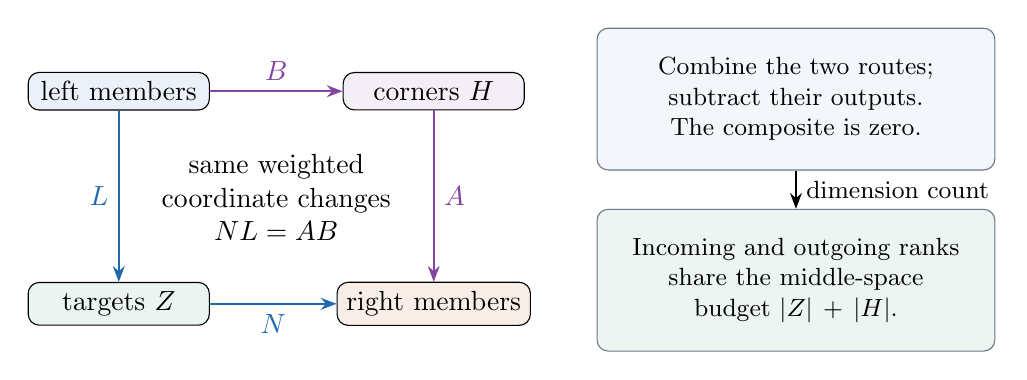
\begin{tikzpicture}
\node[draw,rounded corners,fill=bluefam!9,minimum width=23mm] (r) at (0,0) {left members};
\node[draw,rounded corners,fill=corner!9,minimum width=23mm] (h) at (4,0) {corners $H$};
\node[draw,rounded corners,fill=target!9,minimum width=23mm] (z) at (0,-2.7) {targets $Z$};
\node[draw,rounded corners,fill=orangefam!10,minimum width=23mm] (c) at (4,-2.7) {right members};
\draw[arc,corner] (r)--node[above] {$B$} (h);
\draw[arc,corner] (h)--node[right] {$A$} (c);
\draw[arc,bluefam] (r)--node[left] {$L$} (z);
\draw[arc,bluefam] (z)--node[below] {$N$} (c);
\node[align=center] at (2,-1.35) {same weighted\\coordinate changes\\$NL=AB$};
\node[stage,text width=47mm,fill=soft] (weights) at (8.6,-.1)
{Combine the two routes;\\subtract their outputs.\\The composite is zero.};
\node[stage,text width=47mm,fill=target!8] (budget) at (8.6,-2.4)
{Incoming and outgoing ranks\\share the middle-space\\budget $|Z|+|H|$.};
\draw[arc] (weights)--node[right,font=\small] {dimension count} (budget);
\end{tikzpicture}}

\newcommand{\LegalityPicture}{%
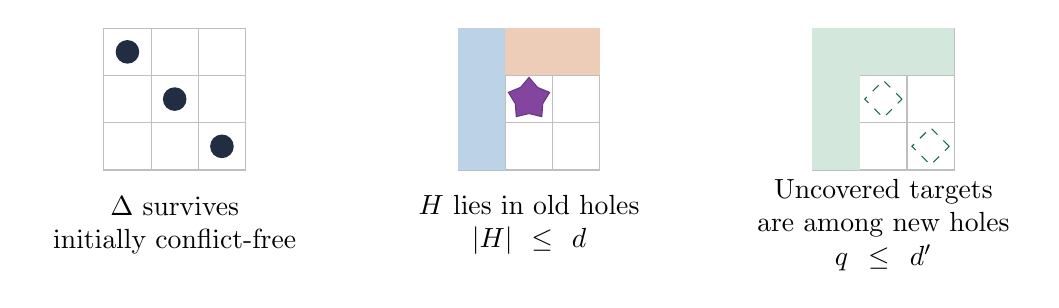
\begin{tikzpicture}
\foreach \shift/\mode in {0/1,4.5/2,9/3}{
\begin{scope}[xshift=\shift cm]
\foreach \i in {0,1,2}\foreach \j in {0,1,2}{\draw[black!25] (\j*.6,-\i*.6) rectangle ++(.6,-.6);}
\ifnum\mode=1
\foreach \i in {0,1,2}{\node[circle,fill=ink,inner sep=0pt,minimum size=3mm] at (\i*.6+.3,-\i*.6-.3) {};}
\node[align=center,text width=35mm] at (.9,-2.5) {$\Delta$ survives\\initially conflict-free};
\else\ifnum\mode=2
\fill[bluefam!30] (0,0) rectangle (.6,-1.8);
\fill[orangefam!30] (.6,0) rectangle (1.8,-.6);
\node[starpt] at (.9,-.9) {};
\node[align=center,text width=35mm] at (.9,-2.5) {$H$ lies in old holes\\$|H|\le d$};
\else
\fill[target!20] (0,0) rectangle (1.8,-.6);
\fill[target!20] (0,-.6) rectangle (.6,-1.8);
\node[targetpt,fill=white,dashed] at (.9,-.9) {};
\node[targetpt,fill=white,dashed] at (1.5,-1.5) {};
\node[align=center,text width=35mm] at (.9,-2.5) {Uncovered targets\\are among new holes\\$q\le d'$};
\fi\fi
\end{scope}}
\end{tikzpicture}}

\newcommand{\LedgerPicture}{%
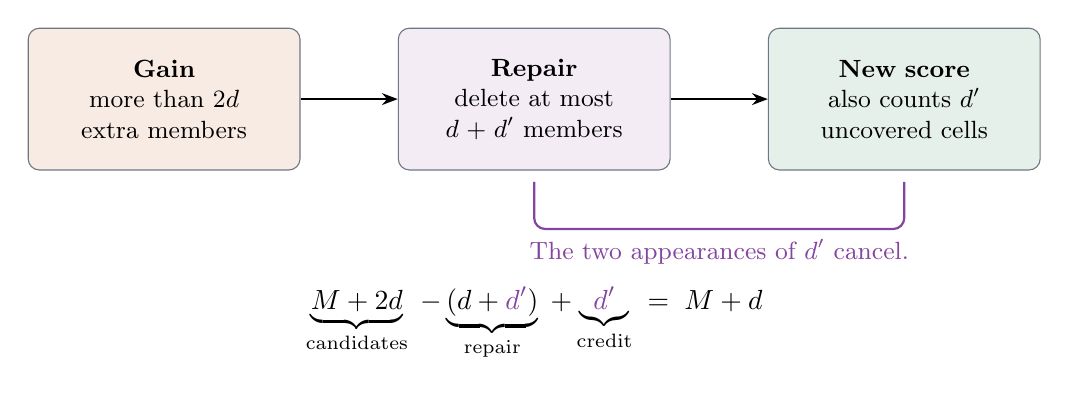
\begin{tikzpicture}
\node[stage,fill=orangefam!12,text width=31mm] (gain) at (0,0)
{\textbf{Gain}\\more than $2d$\\extra members};
\node[stage,fill=corner!10,text width=31mm] (cost) at (4.7,0)
{\textbf{Repair}\\delete at most\\$d+d'$ members};
\node[stage,fill=target!12,text width=31mm] (credit) at (9.4,0)
{\textbf{New score}\\also counts $d'$\\uncovered cells};
\draw[arc] (gain)--(cost);\draw[arc] (cost)--(credit);
\draw[corner,thick,rounded corners] (4.7,-1.05)--(4.7,-1.65)--node[below,font=\small] {The two appearances of $d'$ cancel.} (9.4,-1.65)--(9.4,-1.05);
\node at (4.7,-2.85) {$\underbrace{M+2d}_{\text{candidates}}\;-
\underbrace{(d+\textcolor{corner}{d'})}_{\text{repair}}\;+
\underbrace{\textcolor{corner}{d'}}_{\text{credit}}\;=\;M+d$};
\end{tikzpicture}}

\title{Finding a second neighborhood}
\subtitle{The main ideas of the supplied OpenAI proof}
\author{Codex exposition}
\date{A visual twenty-minute talk}
\begin{document}

\begin{frame}
\titlepage
\vspace{-8mm}
\begin{center}\small
\textcolor{bluefam}{Compare}\quad$\longrightarrow$\quad
\textcolor{orangefam}{Amplify}\quad$\longrightarrow$\quad
\textcolor{target}{Improve}
\end{center}
\note{0:00--0:15. This is an explanation of the supplied September 23, 2026 OpenAI preprint. The mathematical question is local, but the proof goes through subsets and then pairs of subsets on a grid. We will follow the constructions and their purposes. The separate technical deck retains the rank calculations.}
\end{frame}

\begin{frame}{The question: can the second neighborhood catch up?}
An oriented graph has no loops and no opposite pair of arcs.
\begin{center}\NeighborhoodPicture\end{center}
\begin{block}{The theorem}
Every nonempty finite oriented graph has a vertex $v$ with
$|N_1^+(v)|\le |N_2^+(v)|$.
\end{block}
\note{0:15--1:30. Start with the picture. First means one arc; second means shortest directed distance exactly two. Count vertices, not walks. At v there are two first neighbors and one second neighbor. The graph is not a counterexample because c is a sink. The theorem asks for one good vertex, not for all vertices to work. This graph will return in the deletion illustration.}
\end{frame}

\begin{frame}{Three transformations expose the contradiction}
\begin{center}\ProofMap\end{center}
\takeaway{The final move builds a better object than an object chosen to be best.}
\note{1:30--2:15. Assume every vertex fails. Minimum order and then minimum arc count give a set deficit. A transitive-tournament blowup turns the deficit into strict concavity for every nonempty proper subset. The last stage optimizes a pair of families on a grid. Concavity makes a larger candidate; pruning repairs it. The proof is finished if repair costs less than the gain measured by the chosen score.}
\end{frame}

\begin{frame}{Minimality gives a useful before-and-after comparison}
Choose a counterexample with the fewest vertices, then the fewest arcs.
\begin{center}\DeletionPicture\end{center}
\takeaway{Fewer arcs guarantee a good vertex. Compare what that vertex lost and gained.}
\note{2:15--3:30. The displayed graph is a local illustration, not a counterexample: its sink already works. In the hypothetical minimum counterexample, deleting at least one arc preserves orientation and nonemptiness, so arc minimality guarantees some good vertex. If its first neighborhood had not changed, its second neighborhood could only shrink: deleting arcs cannot create two-step paths, and the excluded first neighbors would be unchanged. Therefore the witness loses a first neighbor. For a fixed S, delete arcs from S to the as-yet-unprocessed part of F(S) outside S. The witness lies in S and the lost neighbors form a nonempty batch Q. Vertex minimality also implies strong connectivity, giving positive indegrees and an outgoing arc from every nonempty proper S.}
\end{frame}

\begin{frame}{Process the exterior neighbors in batches}
Put $F(S)=\{y:x\to y\text{ for some }x\in S\}$; let $F^2=F\circ F$.
\begin{center}\scalebox{.9}{\BatchPicture}\end{center}
\[
 |F^2(S)\setminus F(S)|<|F(S)\setminus S|
 \qquad(\varnothing\ne S\subsetneq V).
\]
\note{3:30--4:30. This is the reduction's key invention: a vertex inequality becomes an inequality for every nonempty proper subset. The strip E is partitioned into the batches produced by repeated deletion comparisons. To track the exact net change, put I=F(S) intersection S and g(T)=|F(T) minus (I union T)|. Start with T empty and add Q each time. The comparison at the good vertex gives g(T union Q)-g(T)<|Q|. A net increment may be negative; the picture makes no positivity assertion. At the end g(E)=|F squared(S) minus F(S)|. Add the strict batch inequalities. Each modified graph is formed from the original graph, rather than by accumulating previous deletions.}
\end{frame}

\begin{frame}{Blowup makes a small deficit dominate the errors}
\begin{center}\BlowupPicture\end{center}
\takeaway{Replace each vertex by a large ordered block: amplify the signal, bound the error.}
\note{4:30--5:45. There are n base vertices and every block is a transitive tournament of size m>n. A base arc gives every arc between the corresponding blocks. The subset deficit is a negative integer, so at most minus one. For a subset U whose block support is proper, its contribution scales by m, whereas the internal-block correction is at most one per block. Thus the total is at most minus m plus n, strictly negative. For full support, use positive indegrees: F(U) and F squared(U) are the full blown-up graph, and the desired expression is |U|-|V|<0. That separate case matters. The drawing shows representative three-vertex blocks, not the value of m used in the proof.}
\end{frame}

\begin{frame}{What the reduction has produced}
A nonempty oriented graph with positive indegrees and, for every
nonempty proper $U$,
\[
 |U|+|F^2(U)|<2|F(U)|.
\]
\begin{center}\ConcavityPicture\end{center}
\takeaway{We must show that this uniform drop in set expansion is impossible.}
\note{5:45--6:30. Read the inequality as second increment smaller than first increment, without claiming either increment is positive. F is a set image: it does not remove U. The three boxes are stages, not disjoint sets. A single application of the inequality does not contradict anything. We need to use many sets at once and make orientation participate in the argument. This motivates the grid.}
\end{frame}

\begin{frame}{Why a grid? Orientation becomes disjoint coverage}
A cell $(i,j)$ records a pair. $F_1$ moves its row; $F_2$ moves its column.
\begin{center}\WhyGridPicture\end{center}
\takeaway{The two images of the diagonal meet exactly when opposite arcs exist.}
\note{6:30--8:00. This adapts the useful motivation in Claude's November 14 update. The example is the directed cycle 1 to 2 to 3 to 1. Black dots are the diagonal, which belongs to both families as separate copies. F1 changes the first coordinate vertically: from (1,1) it reaches (2,1). F2 changes the second coordinate horizontally: from (1,1) it reaches (1,2). A shared cell (i,j) would require j to i and i to j. Thus orientation says the diagonal pair starts compatible. For general families, compatibility means their coordinate images are disjoint. Concavity still acts on each column for F1 and each row for F2. This is why pairs simultaneously encode orientation and make the subset inequality reusable. The cycle illustrates the dictionary; it is not the graph with impossible concavity.}
\end{frame}

\begin{frame}{What makes a pair worth keeping?}
$P,Q$ are two sets of grid cells; their images must be disjoint.
\begin{center}\ScorePicture\end{center}
\small The diagonal keeps every relevant line nonempty. Positive indegrees
and compatibility keep those lines proper.
\takeaway{Reward members and uncovered cells: both will pay for the next move.}
\note{8:00--9:15. P and Q are sets of grid points, counted as separate families. Family members are not their images. The colored marks in the board show the images; the black diagonal dots show the members in this example. For the three-cycle, M is six and the three diagonal cells are uncovered by the images, giving score nine. It is just an admissible example, not a claim about a maximizer. In the proof choose a pair containing the diagonal, with disjoint images, maximizing M+d. The board has finitely many cells, so a maximum exists. Each left column contains its diagonal point; each right row does too. If a left column were full, positive indegrees would fill its image column, which meets the other image of the diagonal. Similarly for rows. Hence concavity is applicable to all these lines.}
\end{frame}

\begin{frame}{The planned improvement has one obstruction}
\begin{center}\ImprovementPicture\end{center}
\takeaway{Concavity creates a gain. The new conflicts are the price of realizing it.}
\note{9:15--10:15. Apply concavity to all left columns and right rows, and sum. Replace the left family by the complement of the right second image, and the right by the complement of the left second image. These candidates have more than M+2d members in total. This does not say that either family contains its old version. They need not be compatible. We need to remove conflicts while preserving the diagonal, and the total price must be measured in the same score as before. The pruning lemma is exactly that repair tool.}
\end{frame}

\begin{frame}{Every conflict has two different corner sets}
\begin{columns}[c]
\begin{column}{.54\textwidth}
\centering\RectanglePicture
\end{column}
\begin{column}{.43\textwidth}
\textcolor{target!80!black}{$Z$}: all common targets $z$.\\[8pt]
\textcolor{corner}{$H$}: all opposite corners $h$.
\medskip
\begin{block}{Pruning lemma}
Remove conflicts, retain initially conflict-free members, and achieve
\[
 \#\text{deleted}\le |H|+q,
\]
where $q$ counts targets in $Z$ left uncovered \emph{after} pruning.
\end{block}
\end{column}
\end{columns}
\note{10:15--11:30. A left r=(p,j) and a right c=(i,s) conflict when p to i and s to j. In this picture both coverage arrows are forward set images; they meet at z=(i,j). The other corner h=(p,s) records the same conflict, but is not its common target. H and Z collect corners, not edges with multiplicity. Many conflicts can share a corner. The tool is valid for arbitrary finite relations, even with loops or opposite arcs. q refers only to the original conflict targets Z, not to every hole in the board. The cost is output-dependent; we are not minimizing the number deleted.}
\end{frame}

\begin{frame}{Deleting more can be the right trade}
\small Base arcs: $0\to1,\ 0\to2$. Left: $r_1=(0,1),r_2=(0,2)$;
right: $c_1=(1,0),c_2=(2,0)$. Here $|H|=1$, $|Z|=4$.
\medskip
\begin{center}\PruningExamplePicture\end{center}
\small Crosses mean deleted members. Thin lines are original conflicts.
Hollow diamonds are uncovered targets.
\takeaway{The useful pruning balances deletions against what the survivors leave uncovered.}
\note{11:30--13:00. This star example is already in our article and appears in the other rewrites; Claude's exchange-rate explanation makes it especially effective in a talk. Every left member conflicts with every right member. The sole H point is (0,0), and Z is {1,2} squared. If we delete the entire right side, both left members remain and cover all four targets. Two deletions and q zero fail the desired inequality. If we retain only r1=(0,1), it covers the two cells in column 1 of the target board; the two cells in column 2 are uncovered. Three deletions equal |H|+q=1+2. All members were originally in conflict, so no preservation condition is violated. The two target boards share the same row/column convention as earlier. This is an actual oriented relation, but no claim is made that it satisfies the impossible concavity assumption.}
\end{frame}

\begin{frame}{Survivors pay part of the cover bill}
\begin{center}\CoverPicture\end{center}
\small Add two copies of each $z\in Z$ to the bipartite conflict graph.
A suitable cover has size at most $|H|+|Z|$.
\[
 \#\text{deleted}\le (|H|+|Z|)-(|Z|-q)=|H|+q.
\]
\note{13:00--14:30. A vertex cover meets every undirected edge of the augmented bipartite graph. Its sides are left originals together with left copies of Z, versus right originals together with right copies. Connect originals if they conflict, and connect each original to the opposite copy of every target it covers. The picture is one local pattern, not all of the graph. The highlighted cover here is {r,zL}: delete the original r; the kept c forces zL into the cover. In the full graph, each covered target forces at least one distinct copy into K. Therefore |Z|-q of the cover budget is spent on copies rather than deleting originals. A minimum cover omits isolated vertices, so originally conflict-free members survive. The substantial theorem still needed is the bound on cover size; that is where algebra enters.}
\end{frame}

\begin{frame}{Why linear algebra enters the pruning proof}
\begin{center}\AlgebraPicture\end{center}
\small These are linear maps on coordinate spaces. Here the second-coordinate
maps $B,N$ run \emph{against} the relation.
\takeaway{Maximum-rank kernels connect this space budget to the matching.}
\note{14:30--16:00. Maximum matching equals minimum vertex-cover size in a bipartite graph. Give coordinate moves weights. The two routes act on different coordinates and have identical products: NL=AB. The horizontal linear maps run backward, unlike the earlier coverage arrows. Claude/Fable's update e7337a2 gives the shorter count drawn here. Combine incoming=(L,B) and outgoing=(N,-A). Their composite is zero, so the incoming image lies in the outgoing kernel. Their ranks share the middle-space dimension |Z|+|H|. Normalize the matching into k original conflict edges and ell,t coverage edges. Simultaneously chosen maximum ranks give incoming rank at least ell and outgoing rank at least t. The hard kernel argument and normalized lifts supply k additional independent incoming directions. Hence the whole matching k+ell+t fits within |Z|+|H|. The kernel principle is that an allowed entry cannot couple nonzero left- and right-kernel coordinates: changing it would increase rank. This counts independent directions, not distinct corners for each conflict. The technical deck and unchanged Lean proof retain the equivalent original rank count.}
\end{frame}

\begin{frame}{Why the repaired pair is a legal competitor}
\begin{center}\LegalityPicture\end{center}
\small These diagrams show the three roles. The same finite optimization
problem applies before and after the move.
\takeaway{Pruning costs at most $|H|+q\le d+d'$.}
\note{16:00--17:15. The first panel represents the diagonal, which remains in both candidate families and is isolated there, so pruning preserves it. A conflict involving a diagonal point would make a forbidden two-step image, contradicting the definition by complements. The middle panel represents H among old uncovered cells. If an H corner were in either old image, following one more arc would put one conflicting candidate in the second image excluded from that candidate family. Hence |H|<=d. Finally the conflict targets left uncovered after pruning are among all newly uncovered cells, so q<=d'. The panels are local schematics, not enumerated graphs. They justify both admissibility and the cost bound. The new pair has disjoint images by pruning and contains the diagonal, so its score can be compared with the original maximum.}
\end{frame}

\begin{frame}{The score pays exactly the repair cost}
\begin{center}\LedgerPicture\end{center}
\takeaway{The actual gain is strict, so the new score exceeds the chosen maximum.}
\note{17:15--19:00. Walk through the three cards before the formula. Summed concavity and the complements give more than M+2d candidates. The cost is at most d+d'. Counting uncovered cells in the new objective returns d'. The line on the slide is the cancellation threshold; because the first gain is strict, the real new score is strictly greater than M+d. No comparison between d and d' is assumed. Why coefficient one? It makes the unknown output term cancel. The board is finite, a best admissible pair exists, and the legal improvement contradicts its maximality. Thus no graph produced by the reduction can exist; the initial assumption that all vertices fail is impossible.}
\end{frame}

\begin{frame}{Three ideas to take away}
\begin{center}\ProofMap\end{center}
\begin{enumerate}
\item Compare a minimal obstruction with a simpler version.
\item Amplify a strict integer margin until bounded errors cannot hide it.
\item Count uncovered points so that repairing a better candidate pays for itself.
\end{enumerate}
\medskip
\footnotesize Source: supplied OpenAI preprint, September 23, 2026.
Grid motivation and exchange-rate presentation adapted from the other rewrites;
see \texttt{slide-revision.md}. Full calculations: \texttt{talk-technical.pdf}.
\note{19:00--20:00. Ask the audience to remember the three transformations and, within the final stage, the grid, the repair and its refund. Algebra is the proof of the repair guarantee; it is not the motivation for the extremal objective. The article retains every mathematical detail and explains the weighted and cycle consequences. The separate technical deck retains the previous rank-focused presentation. The project also includes a complete attributed reference Lean proof by Claude Opus 5.5, rebuilt locally, plus independent Codex component checks; this visual revision does not alter their mathematical scope.}
\end{frame}
\end{document}
